\documentclass[aspectratio=1610]{beamer}
\usepackage[utf8]{inputenc}
\usepackage[T1]{fontenc}
\usepackage[german]{babel}
\usepackage[useregional]{datetime2}
\usepackage[nameinlink]{cleveref}
\usepackage[section]{placeins}
\usepackage{xcolor}
\usepackage{graphicx}
\usepackage{csquotes}
\usepackage{amsmath} % for $\text{}$
\usepackage{enumitem}
\setlist{nosep}


\newcommand\urlpart[2]{$\underbrace{\text{\texttt{#1}}}{\text{#2}}$}
\raggedbottom
\crefname{figure}{Abb}{Abb}

\newcommand\producttitle{treff.}
\hypersetup{
	pdftitle={Implementierung: \producttitle},
	bookmarks=true,
}


% header & footer
\usepackage{scrlayer-scrpage}
%\lofoot{\today}
%\refoot{\today}
\pagestyle{scrheadings}

\title{
\includegraphics[width = 50mm]{images/logo_crop.png}}
\subtitle{\huge Implementierung}
\author{Lukas Dippon
	\and Jens Kienle
	\and Matthias Noll
	\and Fabian Röpke
	\and Tim Schmidt
	\and Simon Vögele}

\begin{document}

	\begin{frame}[plain]
	\maketitle
	\end{frame}

	\begin{frame}[plain]
		\frametitle{Entwurf}

		\begin{minipage}{0.5\textwidth}
		placeholder (image)
		\end{minipage}%
		\begin{minipage}{0.5\textwidth}
		\textbf{Freundschaftsanfragen}
		\begin{itemize}
			\setlength\itemsep{0.3em}
			\item[--] ungewollter Kontakt zu Fremden soll vermieden werden
			\item[--] placeholder
		\end{itemize}
		\end{minipage}

	\end{frame}

	\begin{frame}[plain]
		\frametitle{Klient - State}
		\textbf{Funktionsweise}
		\begin{itemize}
			\setlength\itemsep{0.3em}
			\item[--] \textbf{class State:} Wrapper für ViewCall und int
			\item[--] \textbf{enum ViewCall:} mögliche Anfragen an Context
			\item[--] \textbf{SingleLiveEvent:} Observable, wartet auf 
			genau einen Listener
			\item[--] \textbf{in ViewModel:} setValue des state
			\item[--] \textbf{in Activity:} observe des state um UI-Aufrufe 
			zu starten
		\end{itemize}
	$\Rightarrow$ verhindert Aufrufe auf gelöschte Views \\
	$\Rightarrow$ verhindert starke Kopplung zwischen ViewModel und View
	\end{frame}

	\begin{frame}[plain]
	\frametitle{Klient - RequestEncoder}
	\textbf{Fassade für Commands}
	\begin{itemize}
		\setlength\itemsep{0.3em}
		\item[--] Entkopplung der Commands
		\item[--] Einheitliches Verhalten
		\item[--] werden als Queue abgearbeitet
 	\end{itemize}
	\end{frame}

	\begin{frame}[plain]
	\frametitle{Klient - Repositories}
	\begin{figure}[h]
		\centering
		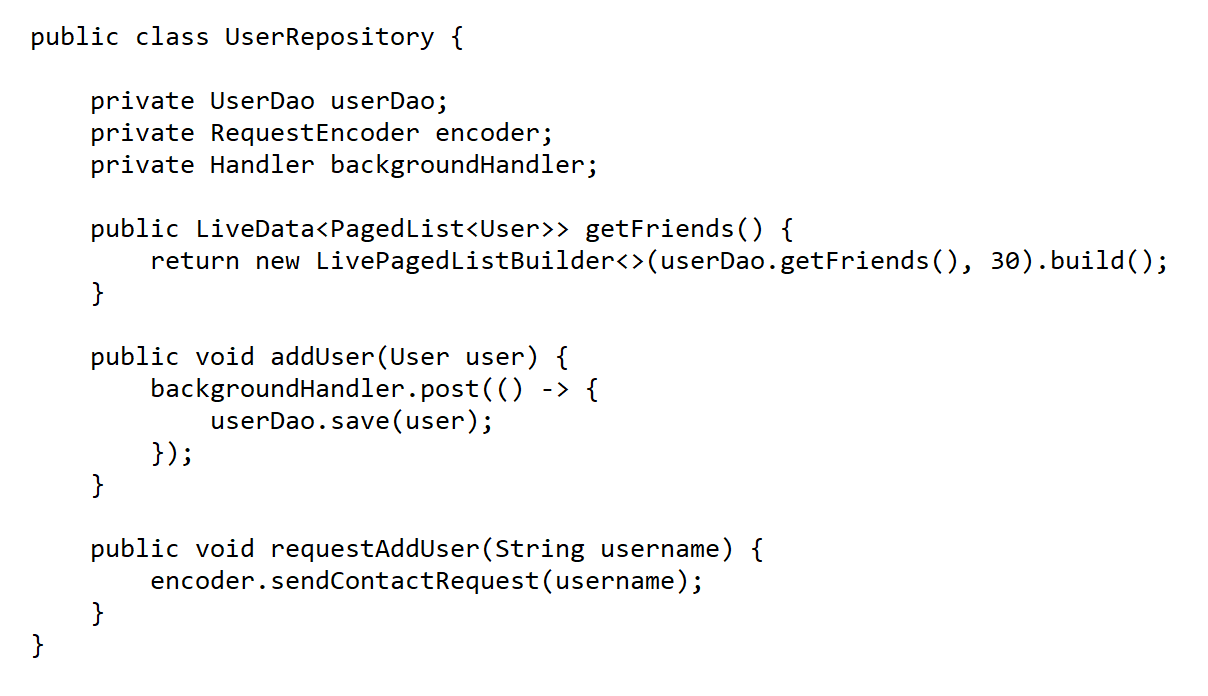
\includegraphics[width=0.8\textwidth]{images/UserRepository.PNG}
		\caption{getrennte Methoden für ViewModels und Encoder}
	\end{figure}
	\end{frame}

	\begin{frame}[plain]
		\frametitle{Server}

	\end{frame}

	\begin{frame}[plain]
		\frametitle{API}

	\end{frame}

\end{document}
